\documentclass[a4paper,12pt]{article}

% ----------------------------------
% Paketi za slovenščino in znanstveno pisanje
% ----------------------------------
\usepackage[slovene]{babel}
\usepackage[utf8]{inputenc}
\usepackage[T1]{fontenc}

% ----------------------------------
% Oblika strani
% ----------------------------------
\usepackage{geometry}
\geometry{margin=2.5cm}

% ----------------------------------
% Matematični simboli in formule
% ----------------------------------
\usepackage{amsmath, amssymb}

% ----------------------------------
% Slike in tabele
% ----------------------------------
\usepackage{graphicx}
\usepackage{caption}
\usepackage{subcaption}
\usepackage{booktabs} % lepe tabele

% ----------------------------------
% Koda (če jo želiš prikazati)
% ----------------------------------
\usepackage{listings}
\usepackage{xcolor}
\lstset{
    basicstyle=\ttfamily\small,
    backgroundcolor=\color{gray!10},
    frame=single,
    breaklines=true
}

% ----------------------------------
% Naslov
% ----------------------------------
\title{\Huge \textbf{Ultimate Texas Hold'em} \\[0.5em]
\Large Poročilo projekta pri predmetu \\[0.2em]
\textit{Izbrane teme iz analize podatkov}}
\author{\Large Neo Mistral \and Oskar Težak \\[1em]
Fakulteta za matematiko in fiziko \\ Univerza v Ljubljani}
\date{\today}

\begin{document}

\begin{titlepage}
    \centering
    \vspace*{3cm}
    
    {\Huge \bfseries Ultimate Texas Hold'em \par}
    \vspace{0.7cm}
    {\Large Poročilo projekta pri predmetu \par}
    \vspace{0.3cm}
    {\LARGE \textit{Izbrane teme iz analize podatkov} \par}
    
    \vfill
    
    {\Large Neo Mistral \\ Oskar Težak \par}
    \vspace{0.5cm}
    {\large Fakulteta za matematiko in fiziko \\ Univerza v Ljubljani \par}
    
    \vfill
    
    {\large \today \par}
\end{titlepage}

\section{Uvod}

Cilj projekta je razviti model z uporabo \textbf{nevronskih mrež}, 
ki bi znal poiskati optimalno strategijo za igranje igre \textit{Texas Hold'em} pokra.

Najboljši in končni rezultati so vključeni v dveh priloženih Jupyter zvezkih:
\begin{itemize}
    \item \texttt{NN-Optim\_Mean.ipynb} \,– končna konfiguracija in rezultati za \textbf{enega igralca} (optimizacija pragov po krogih).
    \item \texttt{NN-Optim\_Mean\_n.ipynb} \,– končna konfiguracija in rezultati za \textbf{$n$ igralcev} (posplošitev na večigralni scenarij).
\end{itemize}

Potek in logika \textbf{generiranja podatkov} sta podrobno dokumentirana v zvezku:
\begin{itemize}
    \item \texttt{data\_generation.ipynb} \,– opis načina vzorčenja, strukturiranja vhodov za posamezne kroge (\emph{pre-flop}, \emph{flop}, \emph{turn}, \emph{river}) in priprava ciljnih spremenljivk (povprečenje, binarni izid, izkupiček posamezne igre).
\end{itemize}

Dodatne pomožne skripte, vmesni poskusi ter spremljevalne datoteke so dostopni v javnem repozitoriju:
\texttt{github.com/oskartezak/Ultimate\_Texas\_Holdem}

Za potrebe projekta sva pravila igre in logiko popolnoma sama implementirala (ultimate.py), 
s čimer sva pridobila popoln nadzor nad generiranjem podatkov in načinom 
prikazovanja igre v simulacijah. V datotetki testiranje.ipynb pa se lahko preiskusi in dobi vpogled v porazdelitev
kombinacij in izid iger pri najini začetni stregiji, katero je cilj izboljšati z uporabo nevronskih mrež.

\section{Opis igre Ultimate Texas Hold'em} 



\textbf{Ultimate Texas Hold'em} je različica pokra, ki se igra proti delilcu, 
ne pa proti drugim igralcem. Cilj igre je premagati delilca z boljšo 
poker kombinacijo iz dveh lastnih in petih skupnih kart.

\subsection*{Potek igre}
\begin{enumerate}
    \item \textbf{Začetna stava} -- igralec postavi enaka vložka na polji \emph{Ante} in \emph{Blind}. 
    Po želji lahko postavi tudi stransko stavo \emph{Trips}, ki se izplača na osnovi končne kombinacije.
    
    \item \textbf{Deljenje kart} -- igralec in delilec prejmeta po dve skriti karti. 
    Igralec lahko zdaj izbere, da stavi dodatno stavo \emph{Play} v višini $3\times$ ali $4\times$ 
    začetne stave, ali pa počaka.
    
    \item \textbf{Flop} -- razkrijejo se prve tri skupne karte. Če igralec prej ni stavil, 
    lahko zdaj postavi stavo \emph{Play} v višini $2\times$ začetne stave, ali pa še vedno počaka.
    
    \item \textbf{Turn in River} -- razkrijeta se še četrta in peta skupna karta. 
    Če igralec do zdaj ni stavil, mora zdaj postaviti stavo \emph{Play} v višini $1\times$ začetne stave.
    
    \item \textbf{Razkritje} -- delilec razkrije svoji dve karti. 
    Za kvalifikacijo mora imeti vsaj par. Če se delilec ne kvalificira, se stava \emph{Ante} vrne igralcu, 
    stave \emph{Blind} in \emph{Play} pa se obravnavajo glede na primerjavo kombinacij.
    
    \item \textbf{Izplačilo} -- 
    \begin{itemize}
        \item Stava \emph{Play} se vedno izplača $1:1$, če je igralčeva kombinacija boljša.
        \item Stava \emph{Ante} se izplača $1:1$, če se delilec kvalificira in igralec zmaga.
        \item Stava \emph{Blind} se izplača po posebni lestvici, odvisno od moči igralčeve kombinacije (npr. \emph{Straight} $1:1$, \emph{Flush} $3:2$, \emph{Full House} $3:1$, ipd.).
        \item Stranska stava \emph{Trips} se izplača posebej glede na moč kombinacije, neodvisno od izida proti delilcu.
    \end{itemize}
\end{enumerate}

\section{Generiranje in oblike podatkov}

Podatke sva generirala naključno. Igra temelji na 52 kartah, ki sva jih označila s številkami od 1 do 52. 
Vsak igralec, vključno z delilcem, prejme dve karti, na mizi pa je skupaj pet kart: najprej trije t.~i.~\textit{flop} 
in nato še dve karti, ki skupaj s prvimi tremi tvorita \textit{river}.

Podatke sva vedno generirala za celotno igro, da sva lahko izračunala njen izid. V model pa sva nato vključila le tiste karte, 
ki so bile na voljo v določenem krogu igre. Te karte so predstavljale vhodne spremenljivke:
\begin{itemize}
    \item v prvem krogu je model videl samo dve karti igralca (ostala mesta so bila nastavljena na 0),
    \item v drugem krogu pet kart,
    \item v tretjem krogu vseh sedem kart.
\end{itemize}

Model nikoli ni imel vpogleda v delilčeve karte. V primeru več igralcev pa je model upošteval tudi njihove karte.

Drugi del podatkov so predstavljale \textbf{ciljne vrednosti}. Preizkusila sva več načinov njihovega določanja:
\begin{enumerate}
    \item \textbf{Povprečenje iger} -- za vsak par igralčevih kart sva generirala več možnih kombinacij preostalih kart in izračunala povprečen izid na 
    za krog igre. 
    \item \textbf{Binaren izid (zmaga/poraz)} -- kot ciljno spremenljivko sva uporabila enostaven pokazatelj zmage ali poraza (0 ali 1). 
    Tudi te vrednosti sva generirala na enak način kot pri povprečenju, le da sva namesto povprečnega izida upoštevala zmago ali poraz.
    \item \textbf{Izkupiček posamezne igre} -- kot ciljno spremenljivko sva uporabila dejanski izid posamezne igre, brez povprečenja. 
    Tudi ti podatki so bili generirani enako kot pri prvem pristopu, pri čemer sva ohranila rezultat posamezne igre.
\end{enumerate}

\paragraph{Velikost podatkovne zbirke.}
Za igralca je velikost podatkovne zbirke znašala 1326 primerov (vseh možnih začetnih kombinacij igralčevih kart). 
Za preostale karte sva uporabila večkratnike te številke: prvi večkratnik $15$ (za "flop"), drugi $15$ (za "river"), 
in pri zadnjem večkratnik $20$ (za delilca). 

\vspace{0.3cm}
\noindent
Očitno za optimalno strategijo v prvem krogu (preflop) ni zares potreben model, saj lahko "profitabilne" začetne roke razberemo direktno iz vzorca, 
ampak v kasnejših krogih (flop, river) postane prostor možnih kombinacij prevelik, zato je uporaba modela smiselna za posploševanje in napovedovanje 
vrednosti tudi za redke ali še nevidene situacije. Kritične so tudi mejne sitiacije, kjer je pričakovan dobiček blizu 0, saj se lahko in se zgodi, da
so nekatere karte bolj "dovzetne" za nekatere kombinacije in dobijo večji potencial v nadaljevanju. Okvirna strategija za preflop je prikazana na nasklednji sliki:

\begin{figure}[h!]
    \centering
    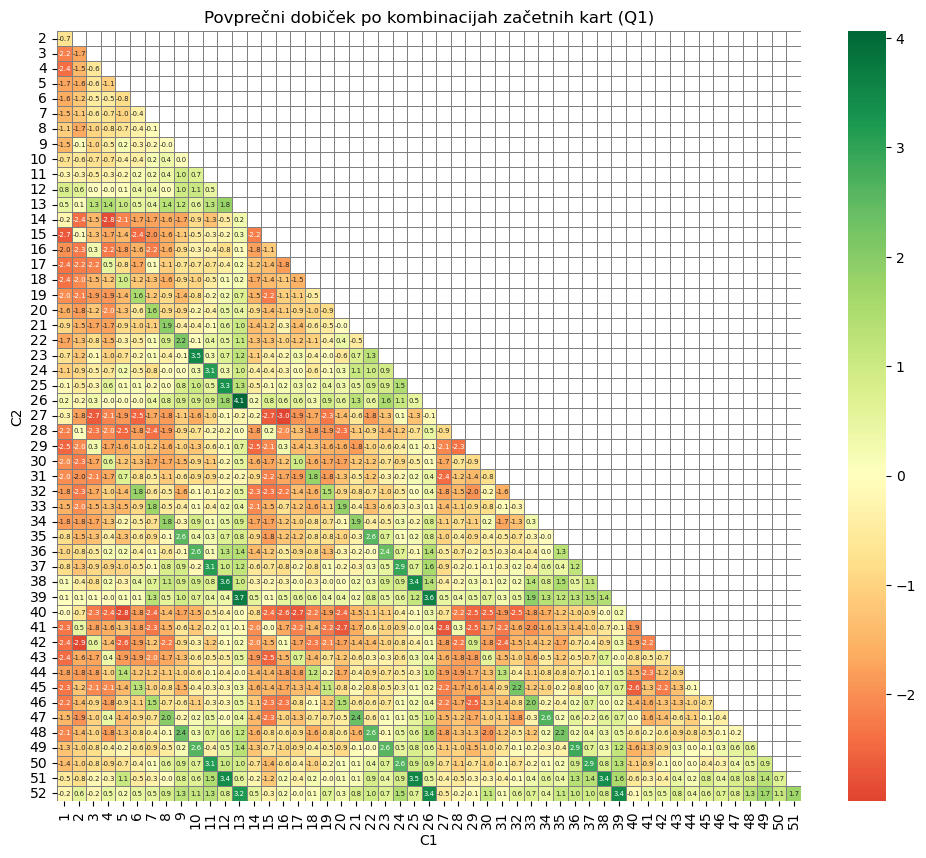
\includegraphics[width=0.8\textwidth]{porazdelitev.png}
    \caption{Prikaz profitabilnosti začetnih kart v prvem krogu (preflop).}
    \label{fig:preflop}
\end{figure}

\section{Metodologija}

Pri večini poskusov sva uporabila \textbf{linearne} oziroma 
\textbf{konvolucijske nevronske mreže}. 
Za določanje stavnih pragov sva poleg različnih optimizacijskih pristopov 
uporabila tudi \textbf{lastne ocene}, s katerimi sva dodatno prilagodila 
strategijo in izboljšala delovanje modela. Povsod sva poskušala z razlčnimi velikostmi
slojev.


\subsection{Poskus 1}
\textbf{Vhodni podatki:} povprečenje iger \\
\textbf{Model:} konvolucijski in linearni modeli z \textit{one-hot} kodiranjem kart \\
\textbf{Rezultati testiranja:} rezultati so bili slabi, modeli niso zaznali uporabnih vzorcev in niso uspeli preseči naključnega ugibanja. \\
\textbf{Komentar:} preveliko število vhodov, ki nosijo premalo informacij. Učenje traja predolgo.

\subsection{Poskus 2}
\textbf{Vhodni podatki:} povprečenje iger \\
\textbf{Model:} konvolucijski in linearni modeli, kjer je bila vsaka karta predstavljena s parom $(\text{rang}, \text{barva})$ \\
\textbf{Rezultati testiranja:} rezultati so bili nezadovoljivi, saj se prednost delilca ni zmanjšala. \\
\textbf{Komentar:} takšna predstavitev slabše prikazuje relacije med kartami.

\subsection{Poskus 3}
\textbf{Vhodni podatki:} povprečenje iger \\
\textbf{Model:} linearni model z \textit{embedding} plastjo in sigmoidno aktivacijsko funkcijo $(0,1)$ \\
\textbf{Rezultati testiranja:} prag za stavo je bil nastavljen na $0.5$. Delilec je v povprečju ohranil prednost približno $5\%$. \\
\textbf{Komentar:} težave pri nastavljanju pragov, model je bil zelo občutljiv na manjše spremembe.

\subsection{Poskus 4}
\textbf{Vhodni podatki:} povprečenje iger \\
\textbf{Model:} konvolucijski model z \textit{embedding} plastjo in sigmoidno aktivacijsko funkcijo $(0,1)$ \\
\textbf{Rezultati testiranja:} prag za stavo $0.5$, delilec je bil v profitu za približno $5\%$. \\
\textbf{Komentar:} enake težave kot pri linearnem modelu – težavno nastavljanje pragov in občutljivost na spremembe.

\subsection{Poskus 5}
\textbf{Vhodni podatki:} binarni izid igre \\
\textbf{Model:} linearni model z \textit{embedding} plastjo in sigmoidno aktivacijsko funkcijo $(0,1)$ \\
\textbf{Rezultati testiranja:} prag za stavo $0.5$. Delilec je ohranil prednost približno $7\%$. \\
\textbf{Komentar:} model ocenjuje le zmage/poraze, ne pa dobička, zato so razlike v izkupičku lahko velike.

\subsection{Poskus 6}
\textbf{Vhodni podatki:} binarni izid igre \\
\textbf{Model:} konvolucijski model z \textit{embedding} plastjo in sigmoidno aktivacijsko funkcijo $(0,1)$ \\
\textbf{Rezultati testiranja:} prag za stavo $0.5$. Delilec je bil v profitu približno $7\%$. \\
\textbf{Komentar:} enake omejitve kot pri linearnem modelu – ocenjevanje le zmage, brez upoštevanja velikosti dobička.

\subsection{Poskus 7}
\textbf{Vhodni podatki:} izkupiček posamezne igre \\
\textbf{Model:} konvolucijski model z \textit{embedding} plastjo in sigmoidno aktivacijsko funkcijo $(0,1)$ \\
\textbf{Rezultati testiranja:} prag za stavo $0.5$. Delilec je bil v prednosti približno $4\%$. \\
\textbf{Komentar:} za enako kakovost rezultatov je potrebna bistveno večja količina podatkov kot pri povprečenju.

\subsection{Poskus 8}
\textbf{Vhodni podatki:} izkupiček posamezne igre \\
\textbf{Model:} linearni model z \textit{embedding} plastjo in sigmoidno aktivacijsko funkcijo $(0,1)$ \\
\textbf{Rezultati testiranja:} prag za stavo $0.5$. Delilec je bil v prednosti približno $5\%$. \\
\textbf{Komentar:} enake ugotovitve kot pri poskusu 7 – potrebna je večja količina podatkov.

\subsection{Poskus 9}
\textbf{Vhodni podatki:} povprečenje iger \\
\textbf{Model:} linearni model z \textit{embedding} plastjo \\
\textbf{Rezultati testiranja:} prag za stavo ročno prilagojen okoli $0$, fiksen za vse kroge. Delilec je bil v povprečju v prednosti približno $4\%$. \\
\textbf{Komentar:} ročno nastavljanje pragov je lažje, model pa se uči razmeroma hitro.

\subsection{Poskus 10}
\textbf{Vhodni podatki:} povprečenje iger \\
\textbf{Model:} konvolucijski model z \textit{embedding} plastjo \\
\textbf{Rezultati testiranja:} prag za stavo ročno prilagojen okoli $0$, fiksen za vse kroge. Delilec je bil v prednosti približno $4\%$. \\
\textbf{Komentar:} podobno kot pri linearnem modelu – enostavnejše nastavljanje pragov in hitrejše učenje.

\subsection{Poskus 11}
\textbf{Vhodni podatki:} binarni izid igre \\
\textbf{Model:} linearni model z \textit{embedding} plastjo \\
\textbf{Rezultati testiranja:} prag za stavo ročno nastavljen okoli $0.5$. Delilec je bil v prednosti približno $5\%$. \\
\textbf{Komentar:} ni velike razlike v primerjavi z uporabo sigmoidne funkcije. Model še vedno ne meri dejanskega dobička.

\subsection{Poskus 12}
\textbf{Vhodni podatki:} binarni izid igre \\
\textbf{Model:} konvolucijski model z \textit{embedding} plastjo \\
\textbf{Rezultati testiranja:} prag za stavo ročno nastavljen okoli $0.5$. Delilec je bil v prednosti približno $6\%$. \\
\textbf{Komentar:} podobno kot pri linearnem modelu – brez merjenja dejanskega dobička, rezultati ostajajo nezadostni.

\subsection{Poskus 13}
\textbf{Vhodni podatki:} izkupiček posamezne igre \\
\textbf{Model:} konvolucijski model z \textit{embedding} plastjo \\
\textbf{Rezultati testiranja:} prag za stavo ročno nastavljen okoli $0$, fiksen za vse kroge. Delilec je bil v prednosti približno $4\%$. \\
\textbf{Komentar:} zaradi velike količine podatkov je bilo učenje počasno.

\subsection{Poskus 14}
\textbf{Vhodni podatki:} izkupiček posamezne igre \\
\textbf{Model:} linearni model z \textit{embedding} plastjo \\
\textbf{Rezultati testiranja:} prag za stavo ročno nastavljen okoli $0$, fiksen za vse kroge. Delilec je bil v prednosti približno $4\%$. \\
\textbf{Komentar:} enake težave kot pri poskusu 13 – prevelik obseg podatkov in posledično počasno učenje.

\subsection{Poskus 15}
\textbf{Vhodni podatki:} povprečenje iger \\
\textbf{Model:} linearni model z \textit{embedding} plastjo \\
\textbf{Rezultati testiranja:} pragovi za vsak krog optimizirani z \texttt{minimize} funkcijo. 
Delilec je bil v prednosti približno $3\%$. \\
\textbf{Komentar:} hitro učenje, optimizator se je izkazal kot učinkovit.

\subsection{Poskus 16}
\textbf{Vhodni podatki:} povprečenje iger \\
\textbf{Model:} konvolucijski model z \textit{embedding} plastjo \\
\textbf{Rezultati testiranja:} pragovi za vsak krog optimizirani z \texttt{minimize} funkcijo. 
Delilec je bil v prednosti približno $3\%$. \\
\textbf{Komentar:} hitro učenje, optimizator se je izkazal kot učinkovit. \\

\vspace{0.5cm}
\noindent
Vsi nadaljni poskusi so bili izvedeni z dvojnim outputom in sicer z pričakovao vrednostjo in standardnim odklonom.
Nova ocenjevana spremnljivka je bil tako \textbf{Sharpe ratio}: $Sharpe = \frac{EV}{std}.$ Izkaže se, da pri malem številu iger pride do
zelo velike variance med posameznimi poskusi, zato je ta pristop (vsaj v teoriji) bolj robusten.

\subsection{Poskus 17}
\textbf{Vhodni podatki:} izkupiček posamezne igre \\
\textbf{Model:} linearni model z \textit{embedding} plastjo \\
\textbf{Rezultati testiranja:} Prednost delilca okoli $6\%$. \\
\textbf{Komentar:} Zelo počasno učenje, težava z batch_size in posledično oceno standardnega odklona.

\subsection{Poskus 18}
\textbf{Vhodni podatki:} izkupiček posamezne igre \\
\textbf{Model:} linearni model z \textit{embedding} plastjo \\
\textbf{Rezultati testiranja:} Pragovi optimizirani z isto mrezo preko soft praga (sigmoid). Prednost delilca okoli $5\%$.\\
\textbf{Komentar:} Soft pragovi se izkažejo kot neučinkoviti, a z hard mejami to ni izvedljivo (ni diferenciabilnosti).

\subsection{Poskus 19}
\textbf{Vhodni podatki:} izkupiček posamezne igre \\
\textbf{Model:} linearni model z \textit{embedding} plastjo in poolingom \\
\textbf{Rezultati testiranja:} Prednost delilca okoli $6\%$.\\
\textbf{Komentar:} Premalo computing power-ja, za tako veliko količino podatkov, zato je bil za občutek pognan na manjšem vzorcu.

\subsection{Poskus 20}
\textbf{Vhodni podatki:} izkupiček posamezne igre \\
\textbf{Model:} linearni model z \textit{embedding} plastjo in poolingom \\
\textbf{Rezultati testiranja:} Enako kot pri 18. Prednost delilca okoli $7\%$.\\
\textbf{Komentar:} Enako kot pri 19.

\subsection*{Primer igranja algoritma}
\begin{verbatim}
Odigranih je bilo 1000 iger
Preflop: 371, Flop: 177, River: 276, Fold: 176
Betted: 20570, Končni proračun: 1100.0
Dobiček: 0.49%
Najvišje stanje: 1255.0 v igri 448
Three of a Kind: 43
Straight: 40
Flush: 27
Full House: 28
Four of a Kind: 1
Straight Flush: 0
Royal Flush: 0
\end{verbatim}

\begin{figure}[h!]
    \centering
    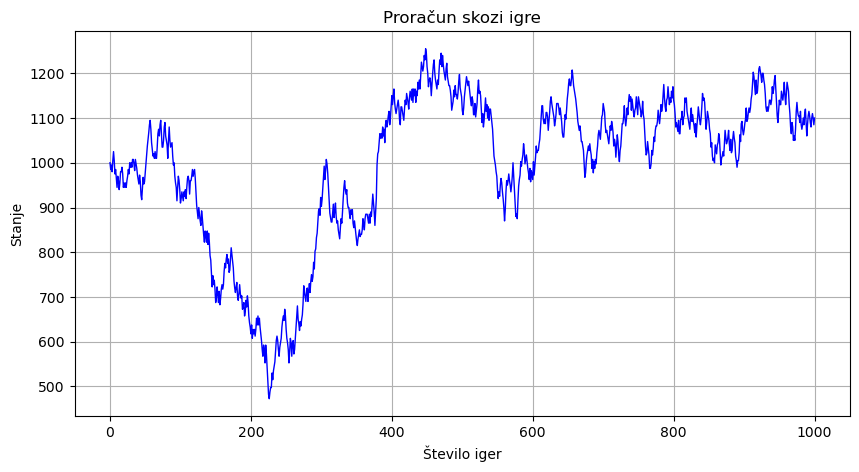
\includegraphics[width=0.8\textwidth]{gibanje.png}
    \caption{Primer igranja algoritma.}
    \label{fig:gib}
\end{figure}


\section{Problemi}

Med izvajanjem projekta sva naletela na več izzivov, ki so pomembno vplivali na kakovost rezultatov in hitrost eksperimentiranja:

\begin{itemize}
    \item \textbf{Vhodna oblika podatkov:} izbira načina predstavitve kart (npr. \textit{one-hot} kodiranje, $(rang, barva)$, 
    \textit{embedding} vektorji) se je izkazala za ključni dejavnik uspešnosti modela. Napačna reprezentacija 
    močno oteži učenje relevantnih relacij.
    
    \item \textbf{Sigmoidna funkcija:} uporaba sigmoidne aktivacijske funkcije je povzročila, da so se vrednosti izhoda 
    pogosto zgoščale v bližini $0$ ali $1$, kar je otežilo stabilno določanje pragov za stave.
    
    \item \textbf{Omejena računska moč:} zaradi omejenih zmogljivosti uporabljenih računalnikov je bilo treniranje 
    modelov počasno, kar je zmanjšalo možnost izvedbe večjih eksperimentov in podrobnejšega iskanja optimalnih nastavitev.
    
    \item \textbf{Čas treniranja:} posamezni poskusi so zahtevali veliko časa za učenje, še posebej pri večjih podatkovnih 
    zbirkah, kar je otežilo iterativno izboljševanje modelov.
    
    \item \textbf{Narava igre:} zasnova igre Texas Hold'em daje dolgoročno prednost delilcu. 
    To pomeni, da model v resnici ne trenira za \emph{zmago}, temveč za zmanjševanje izgub oziroma iskanje 
    strategije, ki vodi v najmanjši možni poraz.
\end{itemize}

\section{Za n igralcev}

\subsection{Podatki}
Za ta sklop poskusov sva uporabila podatke, generirane s \textbf{povprečenjem iger}, 
pri čemer je bilo v simulaciji vključenih \textbf{štiri igralce}. 
Tako kot pri prejšnjih eksperimentih je bil cilj oceniti uspešnost modela pri napovedovanju optimalne strategije.

\subsection{Metodologija}
Metodološki pristop je bil zasnovan podobno kot pri poskusih z enim igralcem. 
Uporabila sva tako \textbf{linearne} kot tudi \textbf{konvolucijske modele}, 
pri čemer sva za določanje stavnih pragov izvedla dodatno \textbf{optimizacijo}. 

\textbf{Rezultati testiranja:} 
Kljub uporabi optimizacije so bili rezultati nezadovoljivi, saj je delilec ohranil 
prednost približno $5.3\%$. 

\textbf{Komentar:} 
Glavni razlog za slabše rezultate je bilo verjetno \textbf{premalo podatkov}, 
da bi model uspel pravilno razbrati vlogo vseh kart in interakcij med več igralci.

\section{Rezultati}

Rezultati eksperimentov kažejo, da uporaba različnih reprezentacij vhodnih podatkov 
(povprečenje iger, binarni izid, izkupiček posamezne igre) ter različnih arhitektur modelov 
(linearni in konvolucijski modeli z \textit{embedding} plastmi) vpliva na končno uspešnost.

\subsection*{Povprečenje iger}
Pri uporabi povprečenja iger so linearni in konvolucijski modeli z \textit{one-hot} 
kodiranjem ali kodiranjem kart kot $(rang, barva)$ dosegali slabe rezultate. 
Modeli niso uspeli izluščiti uporabnih vzorcev, treniranje je bilo dolgotrajno, 
prednost delilca pa se je ohranila na ravni približno $5\%$.

\subsection*{Binarni izid}
Pri prehodu na binaren izid (zmaga/poraz) so modeli dosegali nekoliko stabilnejše napovedi, 
vendar brez izboljšanja končnega rezultata. Delilec je v povprečju obdržal prednost med $6\%$ in $7\%$, 
pri čemer se je izkazalo, da ocenjevanje zgolj zmage brez dejanskega izkupička 
poda popačeno sliko uspešnosti strategije.

\subsection*{Izkupiček posamezne igre}
Pri uporabi dejanskega izkupička posamezne igre so bili rezultati primerljivi, 
a je bila za enako kakovost rezultatov potrebna bistveno večja količina podatkov. 
Delilec je tudi tukaj ostal v prednosti približno $4$--$5\%$.

\subsection*{Optimizacija pragov}
Najboljše rezultate sva dosegla z \textbf{optimizacijo pragov} za posamezne kroge igre 
z uporabo funkcije \texttt{minimize}. V tem primeru je bilo mogoče zmanjšati prednost delilca 
na približno $3\%$. To predstavlja najbolj obetaven pristop, saj kaže, da je z ustrezno optimizacijo 
mogoče nekoliko zmanjšati naravno prednost igre.

\subsection*{Sklepne ugotovitve}
Kljub različnim pristopom in arhitekturam so modeli le delno zmanjšali prednost delilca. 
Najboljši doseženi rezultat je bil približno $3\%$ v prid delilca, kar ne doseže
rezultata, kot sva ga dosegla z lastnimi strategijami.

\subsection*{Nadaljne delo}
V okviru projekta sva poskušala z modeli, ki smo jih spoznali pri tem predmetu, a se je
za konkreten problem izkazalo, da so potrebni bolj specializirani pristopi.
Za nadaljnje delo bova v lastnem režimu razsikala še bolj napredne metode, kot so
\textbf{reinforcement learning} in \textbf{Monte Carlo Tree Search}, ki so se v podobnih problemih izkazale kot zelo učinkovite.
Zadnji korak pa je tudi implementacija igre v spletno aplikacijo, kjer bi lahko model
uporabljali tudi drugi.
Na koncu sva vseeno mnenja, da je bil projekt uspešen, saj sva se naučila veliko novega in pridobila izkušnje z delom na realnem problemu, 
spoznala veliko novih tehnik in orodij ter izboljšala svoje programerske sposobnosti. 
Naučila sva se, da je za dober model potrebno veliko časa in predvsem dobro razumevanje problema,
da se lahko na koncu "izpili" vsaka malenkost za najboljši možni rezultat.

\end{document}
